\chapter{Continuous State Space Models with Discrete Observations}
\label{chap:eight}

The past two chapters have explored different notions of latent
state: a dynamic network in Chapter~\ref{chap:six} and a discrete
latent state in Chapter~\ref{chap:seven}. These notions are a powerful
addition to the autoregressive models of the earlier chapters. In
this chapter, we consider one final extension --- a continuous
latent state that evolves over time. The dynamics of this state will
be conditionally linear, but we will consider a \emph{switching}
variant in which a discrete latent state evolves simultaneously and
governs the choice of linear dynamics rule. By switching between
different linear dynamical regimes, we can obtain highly nonlinear
patterns of dynamics. Moreover, this switching linear dynamical
system will recover a number of common models as special cases. 

The challenge, as should be expected by now, is in performing efficient
inference. Fortunately, at this point we have developed a number of
strategies for tackling this problem. In particular, the \polyagamma
augmentations introduced in Chapter~\ref{chap:five} will make this
problem particularly easy. Once we have augmented our observations
with auxiliary variables, they appear as Gaussian observations to
the latent states. Thus, all of our tools for efficient Bayesian
inference in linear Gaussian models are at our disposal. In particular,
we will derive a block Gibbs sampling algorithm and show that it
outperforms alternative approaches based on Laplace approximations
to the nonconjugate Poisson likelihood.

Finally, we will consider a problem that we have given little
consideration thus far, namely, the problem of Bayesian model
comparison.  We have tacitly assumed that predictive likelihoods
provide a sufficient means of comparing two models. In practice, this
has led to some difficulty, as we encountered with the network model
comparison in Chapter~\ref{chap:five}. The root cause is that
predictive likelihood comparisons only implicitly depend on model
complexity by relying on overfitting to implement a form of Occam's
razor.  In theory, the marginal likelihood --- the denominator in
Bayes' rule --- should provide a better estimate of the trade-off
between how well a model fits the data and the size of the hypothesis
class.

We will show how the fully-conjugate models derived via \polyagamma
augmentation enable principled marginal likelihood estimation
via annealed importance sampling (AIS) \citep{neal2001annealed}. In order
to make this practically feasible, however, we must dive into the
guts of the \polyagamma distribution and develop a novel sampling
algorithm capable of efficiently generating random variates in the
``small shape'' required by AIS. 
 
 
\section{Continuous Latent State Space Models}
Consider a general formulation of models with a continuous latent
state,~$\bx_t \in \reals^D$, with affine and potentially nonstationary
dynamics governed by~$\bA^{(t)}$,~$\bb^{(t)}$, and
covariance,~$\bSigma^{(t)}$. Furthermore, assume that this state
governs the observed spike counts via a linear-nonlinear cascade.  We
summarize this probabilistic model as follows,
\begin{multline}
  p(\bS, \bX \given  \bmu^{(1)}, \{\bA^{(t)}, \bSigma^{(t)}\}, \bC, \{\nu_n\})
  = \\
  \left[
    \distNormal(\bx_1 \given \bmu^{(1)}, \bSigma^{(1)}) \,
    \prod_{t=2}^T \distNormal(\bx_t \given \bA^{(t)} \bx_{t-1} + \bb^{(t)}, \bSigma^{(t)})
  \right] \\
  \left[
    \prod_{t=1}^T \prod_{n=1}^N p(s_{t,n} \given \bc_n \cdot \bx_t, \nu_n)
  \right],
\end{multline}
where
\begin{align*}
  \bC &=
        \begin{bmatrix}
          \text{---} &  \bc_1  & \text{---} \\
            &  \vdots &   \\
          \text{---} &  \bc_N  & \text{---}
        \end{bmatrix} \in \reals^{N \times D}.
\end{align*}
Now consider the special case where there are only~$K$ unique dynamics
and covariance matrices,~${\{\bA^{(k)}, \bb^{(k)}, \bSigma^{(k)}\}}$, and that at
any instant in time, the chosen dynamics are specified by the
discrete latent variable~${z_t \in \{1, \ldots, K\}}$. Moreover,
suppose this discrete latent variable follows a Markov model,
as in the last chapter. Then the dynamics for~$\bX$
are,
\begin{multline}
  p(\bX, \given \bz, \{\bA^{(k)}, \bb^{(k)}, \bSigma^{(k)}\}, \bmu^{(1)})
  = \\ 
    \distNormal(\bx_1 \given \bmu^{(1)}, \bSigma^{(z_1)})
    \prod_{t=2}^T \distNormal(\bx_t \given \bA^{(z_t)} \bx_{t-1} + \bb^{(z_t)}, \bSigma^{(z_t)}),
\end{multline}
with,
\begin{align*}
  p(\bz \given \bpi^{(0)}, \bP) &=
  \distCategorical(z_1\given \bpi^{(0)})
  \prod_{t=2}^T \distCategorical(z_t \given \bpi^{(z_{t-1})}).
\end{align*}
This is known as a \emph{switching linear dynamical system} (SLDS)
model. At any point in time, the latent state obeys linear dynamics.
The particular choice of dynamics switches between~$K$ discrete values
according to a Markov model.

The SLDS contains a number of other models as special cases:
\begin{itemize}
\item When there is only one discrete latent state ($K=1$), this
  reduces to a standard linear dynamical system (LDS).
  
\item When there is one discrete latent state and no continuous dynamics
  (${\bA^{(k)} \equiv 0}$), this reduces to factor analysis (FA).

\item When (i) the state dimensionality is equal to the number of
  neurson~($D=N$); (ii) there are no continuous dynamics (${\bA^{(k)}
    \equiv 0}$); and (iii) the emission matrix is the identity (${\bC
    \equiv \bI}$), the SLDS reduces to a hidden Markov model. At each
  point in time, the firing rate is determined solely
  by~$\bb^{(z_t)}$.

\item When the the conditions of the HMM are met \emph{and} the
  discrete transition matrix,~$P$, has identical rows (${\bpi^{(k)}
    \equiv \bpi}$), the SLDS further reduces to a simple mixture
  model. At each point in time, the discrete latent state is drawn
  from~${z_t \sim \distCategorical(\bpi)}$.
\end{itemize}

\begin{figure}[t]
  \centering%
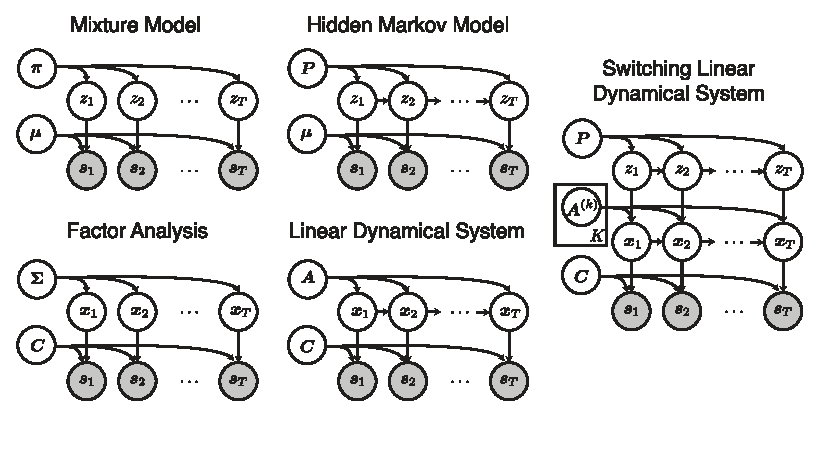
\includegraphics[width=5.5in]{figures/ch8/graphical_models} 
\vspace{-.25in}
\caption{Special cases of the switching linear dynamical system.
  Adapted from Figure~\ref{fig:motifs}.}
\label{fig:slds_models}
\end{figure}

The graphical models corresponding to these special cases are shown in
Figure~\ref{fig:slds_models}, with the omission of some model
parameters to conserve space. This figure is adapted from
Figure~\ref{fig:motifs}. The only model that is not captured here
is the autoregressive model since, here, all interaction between
spike counts arises through the latent state. Next we show how
a single, unified algorithm can support efficient
inference in the SLDS and all its special cases.


\section{Bayesian Inference with \polyagamma Augmentation}

First we show how inference can be performed in the case where
the spikes are imagined to be conditionally Gaussian distributed.
While unrealistic, the key elements of the inference algorithm
will be conserved when we move to discrete count observations.
Given the Gaussian inference algorithm, we will show how the \polyagamma
augmentation explored in Chapter~\ref{chap:five} enables efficient,
fully-conjugate Bayesian inference in discrete models as well.


\subsection{Bayesian Inference with Gaussian Observations}
Suppose the spike counts,~$\bs_t$ were conditionally distributed
according to a Gaussian distribution. Moreover, assume the
distribution has nonstationary, diagonal precision such that
\begin{align}
  \label{eq:gauss_lkhd}
  \bs_{t} &\sim \distNormal(\bC \bx_t, \bOmega_t^{-1}), \\
  \nonumber
  \bOmega_t &= \diag\left( \left[ \omega_{t,1}, \ldots, \omega_{t,N} \right] \right).
\end{align}
In this case, the conditional distribution over continuous latent
states,~$p(\bx_{1:T} \given \bs_{1:T}, \btheta)$, is Gaussian as well.

Specifically, the marginal ``filtered'' distribution,~${p(\bx_t \given
  \bs_{1:t})}$ will be Gaussian. We will write it as,
\begin{align*}
  p(\bx_t \given \bs_{1:t}) &= \distNormal(\bx_t \given \bbm_t, \bV_t).
\end{align*}
We obtain the parameters of this distribution by Kalman filtering.
The following derivations are standard. We follow the presentation of
\citet[Chapter 18]{murphy2012probabilistic}.  Kalman filter consists
of iterating from~${t=1}$ to~${t=T}$. Assume that at iteration~$t$ we
have already computed~$\bbm_{t-1}$ and~$\bV_{t-1}$. Given the
Markovian structure of the probabilistic model, the
conditional distribution of~$\bx_t$ factors into,
\begin{align*}
  p(\bx_t \given \bs_{1:t})
  &\propto
  \underbrace{p(\bs_t \given \bx_t)}_{\text{condition}} \,
  \underbrace{p(\bx_{t} \given \bs_{1:t-1})}_{\text{predict}}.
\end{align*}
To compute its paramters, we perform two steps: we \emph{predict} its
value given preceding observations, and then we
\emph{condition} on the current observation. The predictive
distribution is found by marginalizing over the previous state,
\begin{align*}
  p(\bx_t \given \bs_{1:t-1})
  &\propto  \int p(\bx_t \given \bx_{t-1}) \, p(\bx_{t-1} \given \bs_{1:t-1}) \, \mathrm{d} \bx_{t-1} \\
  &= \distNormal(\bx_t \given \bbm_{t|t-1}, \bV_{t|t-1}),
\end{align*}
where
\begin{align*}
  \bbm_{t|t-1} &\triangleq \bA^{(t)} \bbm_{t-1} + \bb^{(t)} \\
  \bV_{t|t-1} &\triangleq \bA^{(t)} \bV_{t-1}\bA^{(t)^\trans} + \bSigma^{(t)}.
\end{align*}
Then, we condition on the current observations,~$\bs_t$, to get the
parameters of the filtered distribution,
\begin{align*}
  \bbm_t &= \bbm_{t|t-1} + \bK_t (\bs_t - \bC \bbm_{t|t-1}) \\
  \bV_t &= (\bI - \bK_t \bC) \bV_{t|t-1},
\end{align*}
where~$\bK_t$ is the ``Kalman gain'' matrix,
\begin{align*}
  \bK_t &\triangleq \bV_{t|t-1} \bC^\trans \left[ \bC \bV_{t|t-1} \bC^\trans + \bOmega_t^{-1} \right]^{-1}.
\end{align*}

Once we have computed the filtered means and covariances for all
time bins, we can sample from the joint distribution over~$\bX$
by applying the chain rule,
\begin{align*}
  p(\bx_{1:T} \given \bs_{1:T}, \btheta)
  &= p(\bx_T \given \bs_{1:T})
  \prod_{t} p(\bx_{t} \given \bx_{t+1:T}, \bs_{1:T}, \btheta) \\
  &\propto p(\bx_T \given \bs_{1:T})
  \prod_{t} p(\bx_t \given \bs_{1:t}) \, p(\bx_{t+1} \given \bx_{t}, \btheta).
\end{align*}
Thus, we can sample in reverse order, starting with~$\bx_T$ and ending
with~$\bx_1$. The conditional distribution of~${\bx_t}$
\begin{align*}
  p(\bx_t \given \bx_{t+1:T}, \bs_{1:T})
  &\propto
  \distNormal(\bx_t \given \bbm_t, \bV_t) \,
  \distNormal(\bx_{t+1} \given \bA^{(t+1)}\bx_{t} + \bb^{(t)}, \bSigma^{(t+1)}),
\end{align*}
which is yet another Gaussian distribution.

Once we have performed a block Gibbs update for~$\bx_{1:T}$, the rest
of the MCMC algorithm is straightforward. We can perform a block Gibbs
update for~$\bz_{1:T}$ in much the same way. The HMM message passing
algorithms of the last chapter are easily extended to handle this
case. Finally, sampling the parameters, like~$\bA^{(k)}$
and~$\bC^{(k)}$, is straightforward as well.  The problem reduces to
one of inference in a Bayesian linear regression model once we
have conditioned on~$\bz$,~$\bx$, and~$\bs$.

\subsection{\polyagamma Augmentation for Discrete Observations}
The conditional distribution of the latent states is only Gaussian
if the observations are as well. Fortunately, we can make the
observations effectively \emph{look} Gaussian by augmenting the
data with \polyagamma auxiliary variables. 
Recall from Chapter~\ref{chap:five} that the \polyagamma augmentation
is an auxiliary variable scheme that applies to models with logistic
link functions \citep{polson2013bayesian}.  This augmentation can be
used to develop Gibbs for models with likelihoods of the form,
\begin{align*}
  \nonumber  p(s_{t,n} \given \psi_{t,n}, \theta)
  &= c(s_{t,n}, \theta) \, \sigma(\psi_{t,n})^{a(s_{t,n}, \theta)} \,
  (1-\sigma(\psi_{t,n}))^{d(s_{t,n}, \theta)} \\
  &= c(s_{t,n}, \theta)
  \frac{(e^{\psi_{t,n}})^{a(s_{t,n}, \theta)}}
       {(1+e^{\psi_{t,n}})^{b(s_{t,n}, \theta)}}.
\end{align*}
These are called \emph{logistic likelihoods} because the latent
variables are transformed by a logistic
function,~${\sigma(\psi)=e^\psi /(1+e^\psi)}$.  Bernoulli, binomial,
negative binomial, and multinomial likelihoods can all be put in this form.

The augmentation is based on an integral identity
derived from the Laplace transform of the \polyagamma distribution.
Specifically, if $p_{\distPolyaGamma}(\pgvar\given b, 0)$ is the
density of the \polyagamma distribution~${\distPolyaGamma(b, 0)}$,
then
\begin{align}
  \frac{(e^{\psi})^a}{(1+e^{\psi})^b}
  &= 2^{-b} e^{\kappa \psi}
  \int_{0}^{\infty} e^{-\pgvar \psi^2 /2} \,
  p_{\distPolyaGamma}(\pgvar \given b, 0) \, \mathrm{d}\pgvar,
\label{eq:pg_identity_new}
\end{align}
where~${\kappa=a-b/2}$. The integral on the right-hand side is the
Laplace transform of the \polyagamma density evaluated at~$\psi^2/2$,
and the left-hand side is the same form found in discrete
distributions with logistic link functions.  Importantly, viewed as a
function of~$\psi$ for fixed~$\pgvar$, the right-hand side is an
unnormalized Gaussian density.  Thus, the identity
in~\eqref{eq:pg_identity_new} transforms a logistic likelihood to a
Gaussian likelihood conditioned on an auxiliary variable,~$\pgvar$.

Now let~$\psi_{t,n} = \bc_n \cdot \bx_t$ be the activation of neuron
$n$ at time~$t$. The likelihood, as a function of~$\bx_t$, is then
proportional to,
\begin{align*}
  p(\bs_t \given \bx_t, \btheta)
  &\propto \prod_{n=1}^N 
  \frac{(e^{\psi_{t,n}})^{a(s_{t,n}, \theta)}}
       {(1+e^{\psi_{t,n}})^{b(s_{t,n}, \theta)}} \\
  &\propto \prod_{n=1}^N 
     e^{\kappa(s_{t,n}, \theta) \psi_{t,n}}
  \int_{0}^{\infty} e^{-\pgvar_{t,n} \psi_{t,n}^2 /2} \,
  p_{\distPolyaGamma}(\pgvar_{t,n} \given b(s_{t,n}, \theta), 0) \,
  \mathrm{d}\pgvar_{t,n}.
\end{align*}
After introducing these auxiliary variables, the likelihood
of is proportional to a multivariate Gaussian distribution,
\begin{align*}
  p(\bs_t \given \bx_t, \bomega_t, \btheta)
  &\propto \prod_{n=1}^N
  \distNormal(\bc_n \cdot \bx_t \given
  \omega_{t,n}^{-1} \kappa(s_{t,n}, \theta), \,
  \omega_{t,n}^{-1}) \\
  &\propto \distNormal(
  \bOmega_t^{-1} \kappa(\bs_t, \theta) \given
  \bC \bx_t, \, 
  \bOmega_t^{-1}),
\end{align*}
where
\begin{align*}
  \bOmega_t &= \diag \left( \left[ \omega_{t,1}, \ldots, \omega_{t,N} \right] \right).
\end{align*}
Note the similarity of this likelihood and the Gaussian likelihood
of~\eqref{eq:gauss_lkhd}. The only difference is that here the
precision is given by the auxiliary variables, and the observations
are a function of both~$s_{t,n}$ and~$\omega_{t,n}$.
Thus, given a set of \polyagamma auxiliary variables, the block Gibbs
updates that we derived for the Gaussian case will apply equally well
to the discrete case.



Moreover, by the exponential tilting property of the \polyagamma
distribution, the conditional distribution of~$\pgvar_n$
is proportional to a \polyagamma distribution:
\begin{align*}
  \nonumber
  p(\pgvar_{t,n} \given \psi_{t,n}, s_{t,n}, \btheta) &
  \propto e^{-\pgvar_{t,n} \psi_{t,n}^2/2}
  p_{\distPolyaGamma}(\pgvar_{t,n} \given b(s_{t,n}, \btheta), \, 0) \\
  &\propto p_{\distPolyaGamma}(\pgvar_{t,n} \given b(s_{t,n}, \btheta), \, \psi_{t,n}).
\end{align*}
These auxiliary variables are conditionally independent of each other,
and hence amenable to block parallel Gibbs sampling.  Efficient
\polyagamma sampling algorithms have been developed for the regimes
typically encountered in Bernoulli, binomial, and negative binomial
models \citep{windle2014sampling}.

%When the shape parameter,~$b(x_n, \theta)$, goes to zero, the
%\polyagamma density reduces to a delta function at zero. 

Thus, our proposed transition operators,~$\mcT_t$, perform three steps, 
\begin{enumerate}
\item sample~$\bz$ from its Gaussian conditional distribution;
\item sample~$\theta$ from its conditional; and
\item sample all~$\pgvar_n$ in parallel from their \polyagamma conditional distributions.
\end{enumerate}

\subsection{Alternative approaches}
\TODO{
Gaussian and can be computed in closed form, and we can leverage a 
host of off-the-shelf inference algorithms. However, when modeling 
discrete spike counts, a Bernoulli, Poisson model is more appropriate. 
In cases where the spike counts are overdispersed, a negative binomial 
model may provide an even better fit. Unfortunately, these discrete models are not 
conjugate with the Gaussian latent states and inference is
considerably more complicated. Substantial work has gone into 
developing approximate inference algorithms for such models \citep{macke2011empirical},
but these methods rely on approximations to the model. 
% The need for model-specific approximations makes it difficult to 
% tweak the model and incorporate additional structure.
Though these approximations are fast and effective in practice, they can yield
asymptotically biased inferences.
Moreover, they often provide only a point estimate of the latent states and
parameters, which does not reveal Bayesian uncertainty estimates or permit
robust model comparison. 
Here, we present a simpler, faster, fully Bayesian set of algorithms that
are easy to compose and extend.
}



\section{Results}

\begin{figure}
\centering
% Top row: \psi's
  \begin{subfigure}[t]{.26\textwidth}
    \centering
    \vskip 0pt
    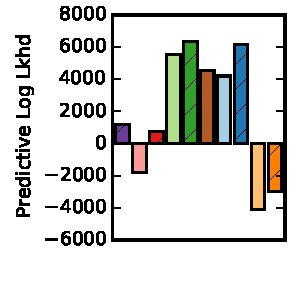
\includegraphics[height=1.4in]{figures/ch8/pred_ll_best_bar.pdf}
    \label{fig:pred_ll_best}
  \end{subfigure}
  ~
  \hspace{-2em}
  \begin{subfigure}[t]{.46\textwidth}
    \centering
    \vskip 0pt
    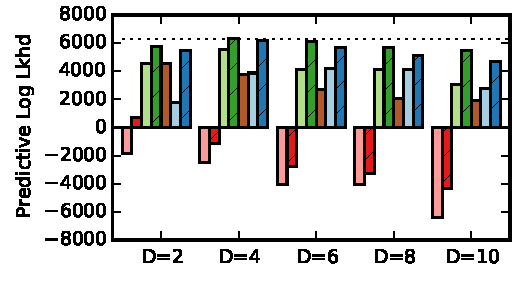
\includegraphics[height=1.4in]{figures/ch8/pred_ll_vs_D_bar.pdf}
  \end{subfigure}
  ~
  \begin{subfigure}[t]{.26\textwidth}
    \centering
    \vskip 0pt
    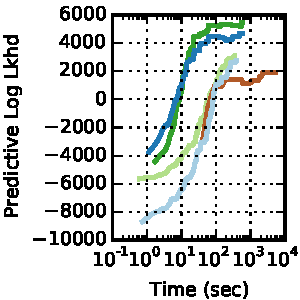
\includegraphics[height=1.4in]{figures/ch8/pred_ll_best_vs_time_D10.pdf}
  \end{subfigure}
  \\
  \begin{subfigure}[t]{\textwidth}
    \centering
    \vskip 0pt
    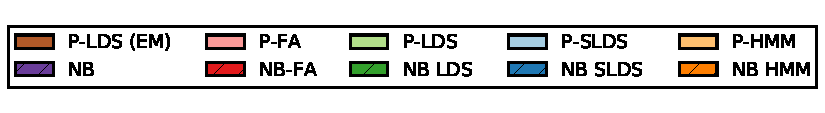
\includegraphics[width=3.8in]{figures/ch8/pred_ll_legend.pdf}
  \end{subfigure}
  \vspace{-1em}
  \caption[Comparison of state space models on hippocampal data]
  {A comparison of latent state space models (FA, LDS, SLDS,
    and HMM) with either Poisson (P) or negative binomial (NB)
    observations fit by our P\'{o}lya-gamma augmented Gibbs sampler to
    a population recording of hippocampal place cells. We measure
    predictive log likelihood on a heldout subset of spike counts and
    find that negative binomial dynamical systems provide the best
    account (left). The latent state space dimensionality,~$D$, is fit
    by cross validation (center), and as the dimension increases the
    models over-fit the training data. Finally, we compare to a
    Poisson LDS (PLDS) model fit via EM and find that our algorithms
    are comparably fast, especially when~$D$ is large
    (right,~$D=10$).}
  \label{fig:hipp8}
\end{figure}


First, we studied a population of 47 hippocampal place cells recorded from a freely moving rat in a 
circular arena.\footnote{Data courtesy of the Wilson lab at MIT.} Spikes were counted in 
250ms bins for approximately ten minutes.
 We held out half of the spike counts (randomly sampled) to compute the predictive 
likelihood of each model relative to a constant-rate Poisson model baseline. 
Figure~\ref{fig:hipp8} shows the results of our comparison for a negative binomial model with constant 
activation and FA, HMM's, LDS's, and switching LDS's with both Poisson and negative binomial observations,
all fit using our augmented MCMC inference algorithm.  We found that the simple FA models over-fit the 
training data and performed poorly on generalization tasks. HMMs, which 
have no low dimensional continuous latent state to tether neurons together, 
performed even worse on predictive tasks. By contrast, the LDS and SLDS 
models and SLDS models exploited temporal dynamics in order to inform latent state estimates.
We explored the effect of the latent state space dimensionality (center panel) and found that 
the LDS and SLDS models generalized well with 4 to 6 dimensional latent states. 
In all cases, the negative binomial 
observation models provided a better fit to the data, suggesting that these 
spike counts were indeed overdispersed (i.e. had variance larger than the mean). With 
our framework, fitting a negative binomial model requires simply changing the 
coefficients of the observation model.

We also compared to a Poisson LDS fit via EM, following \citep{macke2011empirical},
and found that predictive log likelihood estimates with state sequences drawn from 
their variational posterior yield poor predictive estimates. For this dataset, samples 
from our true, non-Gaussian posterior yield more accurate results. Contrary 
to common beliefs about MCMC, our inference algorithms are able to 
explore the posterior parameter space with block Gibbs updates and achieve performance 
that is comparable to EM algorithms, which must solve a large convex optimization problem 
at each iteration (right panel).

Our Bayesian treatment of latent state space models provides a unified 
framework for composing and comparing models of neural activity, and 
identifying latent structure underlying spike trains. As shown with
hippocampal recordings, adopting such an approach allows us to find
a parsimonious description of the neural activity quickly and efficiently
in models that traditionally pose significant inferential challenges.



\section{Marginal Likelihood Estimation}
The marginal likelihood of a model,~$\mcM$, is the probability of the
data,~$\bx$, having integrated out the latent
variables,~$\bz$, and parameters,~$\theta$, of the model:
\begin{align*}
  {p(\bx \given \mcM) = \int p(\bx \given \bz, \theta) \, p(\bz, \theta
  \given \mcM) \, \mathrm{d} \bz \, \mathrm{d}\theta}
\end{align*}
By integrating over the latent variables and parameters, the marginal
likelihood captures a tradeoff between a model's complexity and its
ability to explain the data.  As such, it is a natural criterion for
model comparison. For conjugate exponential family 
models, like linear Gaussian models with Gaussian observations,
 the marginal likelihood can be computed in closed form. 
In these cases, marginal likelihood is often the gold-standard 
for model selection \cite{kass1995bayes}.

Unfortunately, minor adjustments to the model can render the
integration over parameters and latent variables intractable.  For
example, the marginal likelihood is intractable for models with latent
Gaussian structure, like Gaussian processes or linear dynamical
systems, and non-Gaussian observations, like discrete counts.
Instead, we are forced to resort to approximate methods like annealed
importance sampling (AIS) \cite{neal2001annealed}.  AIS is based on
sampling from a sequence of intermediate distributions that
\emph{anneal} between a tractable distribution and the intractable
posterior. While AIS has proven highly effective for a variety of
models \cite{grosse2015sandwiching}, the accuracy of the method hinges
upon the efficiency of the Markov transition operators that target
the intermediate distributions.  Unfortunately, these distributions
often lack exploitable structure present in the posterior, making the
design of efficient transition operators challenging, and ultimately
compromising the efficacy of AIS.

In this work, we develop efficient transition operators that make AIS
simple and efficient for a broad class of models: those in which the
latent variables are Gaussian distributed, the data are discrete, and
the link is provided by a logistic function. Formally, we consider
models of the form,
\begin{align*}
p(\bx, \bz, \theta) 
&= p(\theta) \, \distNormal(\bz \given \bJ_\theta, \bh_\theta) \prod_{n=1}^N p(x_n \given z_n, \theta),
\end{align*}
where the likelihood can be written,
\begin{align*}
\nonumber  p(x_n \given z_n, \theta) &= c(x_n, \theta) \, \sigma(z_n)^{a(x_n, \theta)} \, (1-\sigma(z_n))^{d(x_n, \theta)} \\
  &= c(x_n, \theta) \frac{(e^{z_n})^{a(x_n, \theta)}}{(1+e^{z_n})^{b(x_n, \theta)}}.
\end{align*}
We call these \emph{logistic likelihoods} because the latent variables
are transformed by a logistic function,~${\sigma(z)=e^z /(1+e^z)}$.
Bernoulli, binomial, negative binomial, and multinomial likelihoods
are all in this class.

We have written the Gaussian prior in information form,
\begin{align*}
  \distNormal(\bz \given \bJ_\theta, \bh_\theta) &\propto \exp \left \{-\frac{1}{2} \bz^\trans \bJ_\theta \bz + \bh_\theta^\trans \bz \right\}, 
\end{align*}
which can be related back to the standard form by the
transformations,~$\Sigma = J^{-1}$ and~$\mu = J^{-1}h$.  The Gaussian
prior encapsulates a host of well-known models, like factor analysis,
sparse linear models, Gaussian processes, and linear dynamical
systems, as we will highlight in our applications below.

We begin by reviewing annealed importance sampling and the \polyagamma
augmentation scheme, which we will leverage to develop efficient
transition operators. Section~\ref{sec:pgsampling} derives a
novel sampling algorithm for the \polyagamma distribution --
the main technical contribution of this paper. The remaining
sections illustrate the practical import of this development
by demonstrating significant improvements in marginal likelihood
estimation for a variety of real-world modeling problems.


\subsection{Annealed Importance Sampling}

Annealed importance sampling \cite{neal2001annealed} is a method of
estimating the marginal likelihood,~$p(\bx)$, by ``annealing'' between
a tractable distribution, with known normalization constant, and the
joint distribution, whose normalization constant is the marginal
likelihood of interest. The annealing path is a sequence of
distributions,~${p_1(\theta, \bz), \ldots, p_T(\theta, \bz)}$,
where~${p_t(\theta, \bz)=f_t(\theta, \bz)/\mcZ_t}$,
and~${f_T(\theta, \bz) =p(\theta, \bz, \bx)}$, such that~${\mcZ_T=p(\bx)}$.
Typically, we let~$f_1(\theta, \bz)$ be the normalized prior
distribution such that~${\mcZ_1=1}$. Then, we let~$f_t(\bz, \theta)$ be
a geometric average of the prior and the joint:
\begin{align*}
  f_t(\theta, \bz) &= p(\theta, \bz) \, p(\bx \given \bz, \theta)^{\beta_t},
\end{align*}
with~$\beta_t$ monotonically increasing from~${\beta_1=0}$ to~${\beta_T=1}$.

Given this annealing path, we can generate a sample of~$(\theta,
\bz)$ by first sampling from the prior, and then applying a sequence
of MCMC transition operators~$\mcT_t$ that leave the intermediate
distributions~$p_t$ invariant. The result is a sample that is,
hopefully, closer in distribution to the posterior. We can use
this procedure as a proposal distribution for importance sampling.
The importance weights are given by a product of ratios between~$f_t$ and~$f_{t-1}$.
Since the target density is the unnormalized joint distribution,
the importance weights will be unbiased estimates of the normalization
constant, namely the marginal likelihood,~${\mcZ_T =p(\bx)}$.

How can we reduce the variance of this estimator? First, we can
increase the number of intermediate distributions; second, we can
design rapidly mixing transition operators,~$\mcT_t$. In this work,
we develop transition operators that are both computationally efficient,
allowing us to run more transitions in a fixed amount of time, and more
effective, in that they quickly reach their equilibrium distribution.

With a geometric annealing path, the intermediate distributions are given by,
\begin{align}
  \label{eq:intermediate}
  f_t(\theta, \bz) 
  &= p(\theta) \, \distNormal(\bz \given \bJ_\theta, \bh_\theta) \,  
    \prod_{n=1}^N c(x_n, \theta)^{\beta_t} \frac{(e^{z_n})^{a(x_n, \theta) \cdot \beta_t}}
    {(1+e^{z_n})^{b(x_n, \theta) \cdot \beta_t}}.
\end{align}
There is no immediate conjugacy that we can exploit in order to design
MCMC transition operators for these distributions, but by clever
augmentation, we can derive efficient updates.

However, for this transition to be efficient, 
we must be able to sample from the \polyagamma 
conditional distribution in the regime where~${b(x_n, \theta) \cdot \beta_t < 1}$.
For Bernoulli observations,~${b(x_n, \theta) \equiv 1}$, so we
will be in this regime for all~$\beta_t \in [0,1)$.
While efficient samplers exist for \polyagamma distributed variables 
when the shape parameter is greater than one \citep{windle2014sampling}, 
this ``small shape'' regime has not been previously explored.
We develop a novel sampling algorithm that makes these 
conditional updates extremely efficient, and renders AIS with 
\polyagamma augmented transitions highly effective.

\section{A Novel Sampling Algorithm for the \polyagamma Distribution}
\label{sec:pgsampling}

\begin{figure}
\centering
  \begin{subfigure}[t]{3in}
    \centering
    \vskip 0pt
    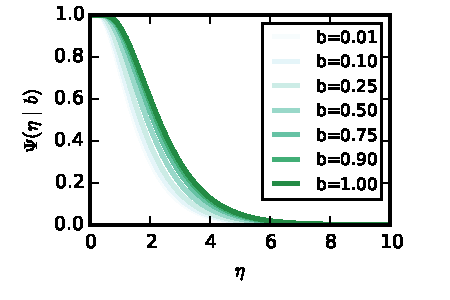
\includegraphics[width=\textwidth]{figures/ch8/psi}
  \end{subfigure}
  \\
  \begin{subfigure}[t]{3in}
    \centering
    \vskip -2em
    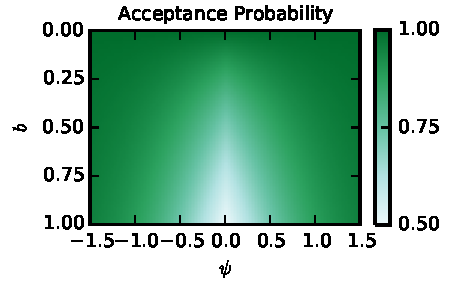
\includegraphics[width=\textwidth]{figures/ch8/acceptance}
  \end{subfigure}
  \vspace{-1em}
  \caption[Rejection sampling algorithm for the \polyagamma
    distribution] {\textit{Top:} Plot of~$\Psi(\pgvar \given b)$, the
    conditional acceptance probability for a proposed value
    of~$\pgvar$, for~$b\in (0,1]$. In all cases, this function is
  monotonically increasing from 0 to 1 as a function of~$\pgvar$, and
  thus defines a cumulative distribution function.  \textit{Bottom:}
  Acceptance probability,~$\alpha(b,z)$, as a function of~$b$
  and~$z$.}
\label{fig:pgsampling}
\end{figure}

The \polyagamma distribution,~$\distPolyaGamma(b,z)$, is closely related 
to the Jacobi distribution,~$\distJacobi(b,z)$, surveyed by \citet{biane2001probability} and 
defined in~\citet{windle2014sampling}.
Specifically, ${\distPolyaGamma(b, z) \sim \frac{1}{4} \distJacobi(b, \tfrac{z}{2})}$.
Thus, to develop a sampler for the \polyagamma distribution, 
it is sufficient to be able to sample the Jacobi distribution.

The density of~$\distJacobi(b,z)$ can be written as an infinite alternating sum,
\begin{multline*}
  p_{\distJacobi}(\pgvar \given b, z) = \\ 
  \cosh^b(z) e^{-\pgvar z^2/2} \frac{2^b}{\Gamma(b)} 
  \sum_{n=0}^\infty (-1)^n \frac{\Gamma(n+b)}{\Gamma(n+1)} \frac{(2n+b)}{\sqrt{2\pi \pgvar^3}}
  \exp\left\{- \frac{(2n+b)^2}{2\pgvar} \right\}.
\end{multline*}
This can be factored as follows,
\begin{align*}
  % \nonumber &p_{\distJacobi}(\pgvar \given b, z) \\
  % \nonumber &\quad= \cosh^b(z) \frac{b 2^b}{\sqrt{2\pi \pgvar^3}} 
  %   \exp \left \{ -\frac{b^2}{2\pgvar} - \frac{\pgvar z^2}{2} \right \}
  %   \Psi(\pgvar \given b) \\
  % &= \cosh^b(z) \frac{b 2^b}{\sqrt{2\pi \pgvar^3}} 
  %   \exp \left \{ -\frac{z^2}{2\pgvar} \left[\left( \frac{b}{z} \right)^2 + \pgvar^2 \right]\right \}
  %   \left( 1-\Psi(\pgvar \given b) \right) \\
  % &= \cosh^b(z) \frac{b 2^b}{\sqrt{2\pi \pgvar^3}} 
  %   \exp \left \{ -\frac{z^2}{2\pgvar} \left[\left( \pgvar- \frac{b}{|z|} \right)^2  +\frac{2b\pgvar}{|z|}\right]\right \}
  %   \left( 1-\Psi(\pgvar \given b) \right) \\
  %&= \cosh^b(z) \frac{b 2^b}{\sqrt{2\pi \pgvar^3}} 
  %  \exp \left \{ -\frac{\left(\tfrac{|z|}{b}\right)^2 b^2}{2\pgvar} \left( \pgvar- \frac{b}{|z|} \right)^2  
  %  -b|z| \right \} 
  %  \left( 1-\Psi(\pgvar \given b) \right) \\
  % &\quad = 2^b \, \cosh^b(z) \, e^{-b|z|} \,
  %   p_{\distInvGaussian} \left(\pgvar \, \bigg| \, \frac{b}{|z|}, \, b^2 \right) 
  %   \Psi(\pgvar \given b),
  p_{\distJacobi}(\pgvar \given b,z) &= 
   \alpha^{-1}(b,z) \,
   p_{\distInvGaussian}\left(\pgvar \, \bigg| \, \frac{b}{|z|}, \, b^2 \right) \,
   \Psi(\pgvar \given b),
\end{align*}
where~$\alpha^{-1}(b,z)$ is a scaling constant greater than one,
\begin{align*}
  \alpha^{-1}(b,z) = 2^b \, \cosh^b(z) \, e^{-b|z|} 
  % &= 2^b \cosh^b(|z|) \, e^{-b|z|} \\
  % &= 2^b \left(\frac{(1+e^{-2|z|}) e^{-|z|}}{2e^{-|z|}} \right)^b \\
  = \left(1 + e^{-2|z|} \right)^b \geq 1;
\end{align*}
where~$p_{\distInvGaussian}(\cdot)$ denotes the inverse Gaussian density,
\begin{align*}
p_{\distInvGaussian} \left(\pgvar \, \bigg| \, \frac{b}{|z|}, \, b^2 \right) 
  % &= \left( \frac{b^2}{2\pi \pgvar^3} \right)^{1/2} 
  %   \exp \left \{ - \frac{b^2 \left(\pgvar - \tfrac{b}{|z|} \right)^2}{2 \left(\tfrac{b}{|z|} \right)^2 \pgvar}   \right \} \\
  &= \frac{b}{\sqrt{2\pi \pgvar^3}}
    \exp \left \{ - \frac{z^2}{2\pgvar}  \left(\pgvar - \frac{b}{|z|} \right)^2   \right \};
\end{align*}
and where we have defined~$\Psi(\pgvar \given b)$ as,
\begin{align*}
  \Psi(\pgvar \given b)  
  &= \sum_{n=0}^\infty (-1)^n \frac{\Gamma(n+b)}{\Gamma(n+1)} \frac{2n+b}{\Gamma(b+1)}
    \exp\left\{- \frac{2n(n+b)}{\pgvar} \right\}.  
\end{align*}
Figure~\ref{fig:pgsampling} plots~$\Psi(\pgvar \given b)$ for various values of~$b$.
% , and shows that it is bounded to the range~$[0,1]$.
Since~$\alpha^{-1}(b,z)\geq 1$ and~$\Psi(\pgvar \given b) \in [0,1]$,
we are guaranteed that~${\alpha^{-1}(b,z)\,
  p_{\distInvGaussian}(\pgvar \given \tfrac{b}{|z|}, b^2)}$
dominates~$p_{\distJacobi}(\pgvar \given b,z)$, which makes the
inverse Gaussian a natural proposal distribution for a rejection
sampling algorithm.  To determine whether a proposed value of~$\pgvar$
is accepted, we must sample~$u \sim \mathrm{Unif}(0,1)$, and check
whether~$u < \Psi(\pgvar \given b)$.
% This is sometimes referred to
% as \emph{generalized rejection sampling}~\cite{devroye1986}.

The acceptance probability is~$\alpha(b,z)$, the inverse of the
scaling constant. It is bounded
between~$[\tfrac{1}{2}, 1]$ when~$b \leq 1$.
The lower bound (worst case) is achieved when~$z=0$ and~$b=1$.
The upper bound (best case) is approached as~$b$ goes to zero or~$|z|$ goes 
to infinity.
This is illustrated in Figure~\ref{fig:pgsampling} for a 
range of~$b$ and~$z$.

Determining acceptance requires a comparison against~$\Psi(\pgvar
\given b)$, for given~$\pgvar$ and~$b$. This function is not
analytically tractable, however, it is still possible to determine
whether or not to accept with finite computation. To do so, we use a
slight modification of the \emph{alternating series method}
\cite{devroye1986}.  We exploit the fact that ~$\Psi(\pgvar \given b)$
is an alternating sum, and the absolute value of the terms is
eventually monotonically decreasing as a function of the index~$n$ for
all fixed values of~$b$ an~$z$.  Thus, after we have computed the
increasing terms, all subsequent partial sums for even~$n$ are upper
bounds, and all subsequent partial sums for odd~$n$ are lower bounds
on~$\Psi(\pgvar\given b)$.  To determine acceptance of~$u$, we
evaluate until we find an upper bound less than~$u$, at which point we
reject, or a lower bound greater than~$u$, at which point we
accept. This is typically done in fewer than six iterations. 
